% !TeX encoding = UTF-8
% !Tex spellcheck = de_DE

%begin:Silbentrennung ****
\RequirePackage{hyphsubst}
\HyphSubstIfExists{ngerman-x-latest}{\HyphSubstLet{ngerman}{ngerman-x-latest}}{} 
\listfiles
%end:Silbentrennung ******

\documentclass[12pt,a4paper]{article}
% ***********************************************************
% ***************** MyStyle - Rene Vollmer*******************
% ***********************************************************
% Version 1.0b



\usepackage[utf8]{inputenc}

\usepackage{hyperref}

\usepackage{amsmath} % AMS Math Package
\usepackage{amsfonts}
\usepackage{amsthm} % Theorem Formatting
\usepackage{amssymb}	% Math symbols such as \mathbb
\usepackage{mathtools}
\usepackage{graphicx} % Allows for eps images
\usepackage{multicol} % Allows for multiple columns
\usepackage[]{units}

\usepackage{hyperref} %Links
\usepackage{url}

\usepackage{verbatim} %Fuer mehrzeilige kommentare \begin{comment} \end{comment}

\usepackage[hang]{caption} % Captions einrücken
\usepackage{subfigure}

%Some other shit
\usepackage{float}
%\floatstyle{boxed} %Puts a box around each figure
\restylefloat{figure}
%\usepackage{wrapfig}
\usepackage{microtype}



\usepackage{xparse} % For uses like \DeclareDocumentCommand{\foocmd}{ O{default1} O{default2} m }{#1~#2~#3}


%\usepackage{color}
%\definecolor{gray}{rgb}{.5,.5,.5}
%\definecolor{lightgray}{rgb}{.25,.25,.25}

%Graphics (PGF / TIKZ) **+**+**+**+**+**+**+**+**+**+**+**+**+**+
\usepackage{tikz}
\usetikzlibrary{patterns}
\tikzset{
	hatchhor/.style={pattern=horizontal lines,pattern color=#1},
	hatchhor/.default=black
}
\tikzset{
	hatchvert/.style={pattern=vertical lines,pattern color=#1},
	hatchvert/.default=black
}
\tikzset{
	hatchdiag/.style={pattern=north east lines,pattern color=#1},
	hatchdiag/.default=black
}
\tikzset{
	hatchdiag2/.style={pattern=north west lines,pattern color=#1},
	hatchdiag2/.default=black
}
%also possible grid, crosshatch, dots, crosshatch dots, fivepointed stars, sixpointed stars

\usepackage{pgfplots}
\usepgfplotslibrary{fillbetween}

% Style to select only points from #1 to #2 (inclusive)
\pgfplotsset{select coords between index/.style 2 args={
		x filter/.code={
			\ifnum\coordindex<#1\def\pgfmathresult{}\fi
			\ifnum\coordindex>#2\def\pgfmathresult{}\fi
		}
	}
}


\newcommand{\vasymptote}[2][]{
	\draw [color=gray,densely dashed,#1] ({rel axis cs:0,0} -| {axis cs:#2,0}) -- ({rel axis cs:0,1} -| {axis cs:#2,0});
}

\newcommand{\vertline}[2][]{
	\draw [#1] ({rel axis cs:0,0} -| {axis cs:#2,0}) -- ({rel axis cs:0,1} -| {axis cs:#2,0});
}
%END Graphics **+**+**+**+**+**+**+**+**+**+**+**+**+**+**+**+**+

%Stolen from http://www.dfcd.net/articles/latex/latex.html
% **#**#**#**#**#**#**#**#**#**#**#**#**#**#**#**#**#**#**#**#**#
\makeatletter % Need for anything that contains an @ command

\let\vaccent=\v % rename builtin command \v{} to \vaccent{}
\renewcommand{\v}[1]{\ensuremath{\mathbf{#1}}} % for vectors
\newcommand{\gv}[1]{\ensuremath{\mbox{\boldmath$ #1 $}}} 
% for vectors of Greek letters
\newcommand{\uv}[1]{\ensuremath{\mathbf{\hat{#1}}}} % for unit vector
\newcommand{\abs}[1]{\left| #1 \right|} % for absolute value
\newcommand{\avg}[1]{\left< #1 \right>} % for average
\let\underdot=\d % rename builtin command \d{} to \underdot{}
\renewcommand{\d}[2]{\frac{d #1}{d #2}} % for derivatives
\newcommand{\niced}[2]{\nicefrac{d #1}{d #2}} % for in-text-derivatives
\newcommand{\nicedd}[2]{\nicefrac{d^2 #1}{d #2^2}} % for double derivatives\newcommand{\dd}[2]{\frac{d^2 #1}{d #2^2}} % for in-text-double derivatives
\newcommand{\pd}[2]{\frac{\partial #1}{\partial #2}} 
% for partial derivatives
\newcommand{\pdd}[2]{\frac{\partial^2 #1}{\partial #2^2}} 
% for double partial derivatives
\newcommand{\pdc}[3]{\left( \frac{\partial #1}{\partial #2}
	\right)_{#3}} % for thermodynamic partial derivatives
\newcommand{\ket}[1]{\left| #1 \right>} % for Dirac bras
\newcommand{\bra}[1]{\left< #1 \right|} % for Dirac kets
\newcommand{\braket}[2]{\left< #1 \vphantom{#2} \right|
	\left. #2 \vphantom{#1} \right>} % for Dirac brackets
\newcommand{\matrixel}[3]{\left< #1 \vphantom{#2#3} \right|
	#2 \left| #3 \vphantom{#1#2} \right>} % for Dirac matrix elements
\newcommand{\grad}[1]{\gv{\nabla} #1} % for gradient
\let\divsymb=\div % rename builtin command \div to \divsymb
\renewcommand{\div}[1]{\gv{\nabla} \cdot #1} % for divergence
\newcommand{\curl}[1]{\gv{\nabla} \times #1} % for curl
\let\baraccent=\= % rename builtin command \= to \baraccent
\renewcommand{\=}[1]{\stackrel{#1}{=}} % for putting numbers above =
\newtheorem{prop}{Proposition}
\newtheorem{thm}{Theorem}[section]
\newtheorem{lem}[thm]{Lemma}
\theoremstyle{definition}
\newtheorem{dfn}{Definition}
\theoremstyle{remark}
\newtheorem*{rmk}{Remark}
% **#**#**#**#**#**#**#**#**#**#**#**#**#**#**#**#**#**#**#**#**#


%Equalssign with hat/corresponds to   \equalhat
\newcommand\equalhat{%
	\stackrel{\Lambda}{=}
}
%Equalssign with !
\newcommand\shallbe{%
	\stackrel{!}{=}
}
% := and =:
\newcommand{\defeq}{\vcentcolon=}
\newcommand{\eqdef}{=\vcentcolon}



%Encirecled Numbers, used in Graphics
\let\depth\relax
\def\X#1{%
	%#1%
	%\textcircled{#1}%
	\raisebox{0.9pt}{\textcircled{\raisebox{-.9pt}{#1}}}%
	%\ding{\numexpr171+#1\relax}%
}


% ******************************~~~~*****************************
%Photo quality management. This is an old try:
\newcommand\openfile{\newwrite\outputstream\immediate\openout\outputstream=photo.log
	\writetofile[linewidth]{\the\linewidth}
	\writetofile[textwidth]{\the\textwidth}
	\writetofile[dpi]{300}
	}
\newcommand\closefile{\immediate\closeout\outputstream}
\newcommand\writetofile[2][2]{\immediate\write\outputstream{#1 #2}}

\newcommand\photo[2][2]{\includegraphics[width=#1]{#2}\writetofile[#2]{#1}}

% ***************************************************************
% And this is working
% Reduce image size for fixed dpi
% Introduce \includegraphicsRS for this purpose

% for downsampling large images: \includegraphicsRS
% (\includegraphics "resize")
% \includegraphicsRS[#1][#2]{#3}
% #1 = normal \includegraphics[] - Parameter (like scale=1) {optional}
% #2 = approx part of the screen, eg half page width use 0.5 or 1/2 {optional}
%      reduces to #2*1000px
% #3 = relative path to image file WITH ending (e.g. .jpg) {required}
\pdfimageresolution 300

\newcommand{\includegraphicsRS}{}

\ifnum\pdfshellescape=1
% Yes, enabled
% IFP - image file path
% IFN - image filename only
% here resizing at #2*1000 px wide
\newread\myinput
% must add default argument [] so typeout works
\DeclareDocumentCommand{\includegraphicsRS}{ O{\@empty} O{1} m }{ %
%\renewcommand\includegraphicsRS[2][\@empty]{
	% run downsampling bash script
	\immediate\write18{mkdir -p images; mkdir -p images/downsampled; IFP=#3 ; %
		PIX=#2 ; PIX=$( awk  'BEGIN { rounded = sprintf("\%.0f", ('$PIX')*1000); print rounded }' ) ;
		echo "$PIX 1000 *p" | dc ; %
		echo "Processing $IFP" ; %
		IFN=$(basename $IFP) ; %
		echo "images/downsampled/$IFN" > tmpname ; %
		if [ ! -f images/downsampled/$IFN ]; then %
		echo "File images/downsampled/$IFN not found! Converting..." ; %
		%the \string> after the pixel width (e.g. 1000x) will prevent imagemagick from producing files larger than the original
		convert $IFP -resize $PIX"x\string>" -quality 85 images/downsampled/$IFN ; %

		else %
		echo "Found images/downsampled/$IFN - reusing." ; %
		fi ; %
		%alternatively: bash includegraphicsRS.sh #3 #2
		%and have the code in the *.sh-file.
	} % end write18
	% here we should have downsampled file
	% retrieve downsample filename first
	\immediate\openin\myinput=tmpname
	% The group localizes the change to \endlinechar
	\bgroup
	\endlinechar=-1
	\immediate\read\myinput to \localline
	% Since everything in the group is local, we have to explicitly make the
	% assignment global
	\global\let\myTmpFileName\localline
	\egroup
	\immediate\closein\myinput
	% Clean up after ourselves
	% \immediate\write18{rm -f -- tmpname}
	% finally, include downsampled image
	\includegraphics[#1]{\myTmpFileName}
} % end renewcommand
\else
% No, disabled
% in this case, \includegraphicsRS is just the usual \includegraphics
\renewcommand\includegraphicsRS[2][\@empty]{%
	\includegraphics[#1]{#2}
}
\fi

\begin{comment}
old stuff, not used any longer. Could be useful for future changes though.
\usepackage{fp}

\newlength{\TOarg} \newlength{\TOunit}
{\catcode`p=12 \catcode`t=12 \gdef\TOnum#1pt{#1}}
\newcommand\TOop[2]{\setlength{\TOarg}{#2}%
	\FPdiv\TOres{\expandafter\TOnum\the\TOarg}{\expandafter\TOnum\the\TOunit}%
	\FPround\TOres\TOres{#1}}
\newcommand{\TOspace}{\ }
\newcommand\TOpt[2][2]{\setlength{\TOunit}{1pt}\TOop{#1}{#2}\TOres\TOspace pt}
\newcommand\TOin[2][2]{\setlength{\TOunit}{1in}\TOop{#1}{#2}\TOres\TOspace in}
\newcommand\TOcm[2][2]{\setlength{\TOunit}{1cm}\TOop{#1}{#2}\TOres\TOspace cm}
\newcommand\TOmm[2][2]{\setlength{\TOunit}{1mm}\TOop{#1}{#2}\TOres\TOspace mm}
\newcommand\TOem[2][2]{\setlength{\TOunit}{1em}\TOop{#1}{#2}\TOres\TOspace em}
\newcommand\TOpx[2][2]{\setlength{\TOunit}{1px}\TOop{#1}{#2}\TOres\TOspace px}
\newcommand\TOptdeux[2][2]{\setlength{\TOunit}{1pt}\TOop{#1}{#2}\TOres}

convert $IFP -resize 50\% images/downsampled/$IFN ; %		textwidth="\the\textwidth" ; %
TW=${textwidth:0:(-2)} ; %
VARI="$TW"; %
convert -resize 2000x -units pixelspercentimeter $IFP -density 120 -pointsize 30 -draw "gravity south-east fill black text 0,5 '$VARI'" downsampled/$IFN ; %
\end{comment}


% END of \includegraphicsRS
% ***************************************************************
% ******************************~~~~*****************************



% ***********************************************************
% ********************** END HEADER *************************
% ***********************************************************
\usepackage[left=2.50cm, right=2.50cm, top=2.50cm, bottom=2.00cm]{geometry}


\usepackage[ngerman]{babel}

%test
\begin{comment}
\usepackage{titlesec}
\titleformat{\subsection}[runin]% runin puts it in the same paragraph
{\normalfont\bfseries}% formatting commands to apply to the whole heading
{\thesubsection}% the label and number
{0.5em}% space between label/number and subsection title
{}% formatting commands applied just to subsection title
[]% e.g. [.] punctuation or other commands following subsection title\frac{•}{•}
\end{comment}

\linespread{1.1}
\usepackage{microtype}

%\addto\captionsgerman{ \renewcommand{\figurename}{\small{\textbf{Abb.}}}
%\captionsetup{figurewithin = section}
%\captionsetup{font=small, labelfont=bf} }


\begin{document}
	
	\pagenumbering{Roman}
	%TODO REMOVE
	%\textbf{TODO}
	%
René
\begin{enumerate}
	\item Regina sagen, dass sie auf die Eigenschaften der FT refen soll
	\item Regine Videos vom Handy geben
	\item Regina Rücktransformierte Bilder geben
	\item 
\end{enumerate}

Vivi
\begin{enumerate}
	\item @ rené: ich hab bei der section "einkopplung" jetzt keine unsrer Leistungs-berechnungs- rechnungen hingeschrieben, weil die ja alle für die photodiode waren, mit irgendwelchen zu großen widerständen... 
	\item ...
\end{enumerate}
	
	
	%Metadaten
	\title{\textit{Fortgeschrittenenpraktikum}\\\textbf{Optische Fouriertransformation} }
	\date{August 2015}
	\author{Vivien Sleziona \footnote{vivi.s@arcor.de}\\ Regina Schauer \footnote{regina.schauer@web.de}\\ René Vollmer \footnote{rene.vollmer@studium.uni-hamburg.de} \\ \\Betreut durch\\ Kai Morgener\footnote{kmorgene@physnet.uni-hamburg.de}}
	
	\maketitle
	
	\begin{center} 
		\bigskip
		\bigskip
		
		\begin{minipage}{0.75\textwidth}
			\textbf{[Zusammenfassung]}
			% !TeX root = ../praktikum.tex
% !TeX encoding = UTF-8
% !Tex spellcheck = de_DE

Die Fourier-Analytik und insbesondere die Fouriertransformation sind auf vielen modernen Anwendungen kaum noch weg zu denken. Sie ist essentieller Bestandteil vieler Bildverarbeitungsalgorithmen\cite{easton_fourier_2010} und -kompressionsverfahren wie JPEG\cite{_jpeg_2015}, sie wird genutzt um Bildinformationen Computeralgorithmen zugänglich zu machen\cite{prof._dr._norbert_link_vorlesungsscript:_????} und in vielen anderen Bereichen der Signalverarbeitung.\\

In diesem Versuch soll mit einfachen optischen Mitteln eine Fouriertransformation auf Bildern durchgeführt, die Fouriertransformierte manipuliert und rücktransformiert werden. Dabei wird dem Leser ein intuitives Verständnis für die Funktionsweise und Bedeutung von Fouriertransformationen vermittelt werden.
		\end{minipage}
	\end{center}
	
	%\vfill
	\newpage
	
	\tableofcontents
	\vfill
	\newpage
	\clearpage	
	
	\pagenumbering{arabic}
	
	\section{Theoretische Grundlagen}
	% !TeX root = ../praktikum.tex
% !TeX encoding = UTF-8
% !Tex spellcheck = de_DE

\begin{align}
	\vec{\j} = \mathbf{\sigma} \cdot \vec{E} & & \Leftrightarrow & & \vec{E} = \mathbf{\rho} \cdot \vec{j}
	\label{eq:u2rho}
\end{align}

	
	\newpage
	\clearpage
	\section{Aufbau und Justage des Experiments}
	Der Aufbau des Versuches für die optische Fouriertransformation bestand aus drei Teilen: Zunächst wurde die Einkopplung des Laserstrahls im Faserkopplungsaufbau optimiert und die Effizienz dieser gemessen. Anschließend wurde die Tauglichkeit einer Photodiode zur Messung der Lichtleistung und somit der Einkoppeleffizienz untersucht. Abschließend wurde hinter dem Auskoppler der für die Erzeugung, Aufnahme und Manipulation der Fourierspektren sowie die Rücktransformation benötigte 4f-Aufbau aufgebaut und optimiert.
	
	\subsection{Einkopplung}
	% !TeX root = ../praktikum.tex
% !TeX encoding = UTF-8
% !Tex spellcheck = de_DE

	\subsection{Lichtsensor}
	% !TeX root = ../praktikum.tex
% !TeX encoding = UTF-8
% !Tex spellcheck = de_DE

Für die Optimierung der Einkopplungsleistung wurde ein Powermeter benutzt. Dieses wurde an ein digitales Oszilloskop angeschlossen, um schnelle Änderungen zu visualisieren und so den Optimierungsvorgang, insbesondere das \textit{Walken}, zu erleichtern. Da diese Powermeter mit recht hohen Anschaffungskosten einher gehen, wurde in diesem Versuchsteil versucht, eine Leistungsmessung des Laserlichtes mit einer Photodiode zu messen.\\

Die verwendete Photodiode\footnote{Modell OSD15-5T von CENTRONIC\cite{farnell.com_osd15-5t_????}} produziert laut Datenblatt einen Strom von \unit[0,18-0,21]{mA} pro Milliwatt eingestrahlter Lichtleistung bei \unit[436]{nm} Wellenlänge. Da Strom nicht direkt gemessen werden kann, wird ein Widerstand parallel geschaltet und der Spannungsabfall über diesen nach $U=R\cdot I$ mit einem Oszilloskop gemessen. Wenn man für \unit[1]{mW} Lichtleistung einen Spannungsabfall von \unit[100]{mV} erreichen möchte, würde man einen $\nicefrac{U}{I}=\nicefrac{\unit[100]{mV}}{\unit[0,2]{mA}}=\unit[500]{\Omega}$ Widerstand verwenden. Da dies jedoch ein sehr kleiner Messbereich ist, wurden \unit[4]{V} pro Milliwatt angesetzt und entsprechend ein \unit[20]{$k\Omega$} Widerstand verwendet.\\

Bei sehr schwachen Lichteinfall (Deckenlampe, Fenster aus der Ferne, ...) konnte auf dem Oszilloskop eine Schwankung in der Spannung festgestellt werden. Bei hohen Lichtleistungen fallen diese Schwankungen sehr klein aus. Für andere Widerstandswerte, z.B. 10 oder \unit[100]{$k\Omega$}, erhält man nahezu identische Werte um \unit[440]{mV}. Da dies in etwa der Bandlücke eines PN-Überganges entspricht, liegt die Vermutung nahe, dass dies eine Sättigungserscheinung ist.

Daher wurde der Aufbau mit kleineren Widerstandswerten von 500 und \unit[1000]{$\Omega$} getestet. Die gemessenen Spannungen sowie die dazu vom Powermeter abgelesenen Werte für die Lichtleistung sind in Abbildung~\ref{fig:photodiode} aufgetragen.


\begin{figure}[ht]
	\centering
	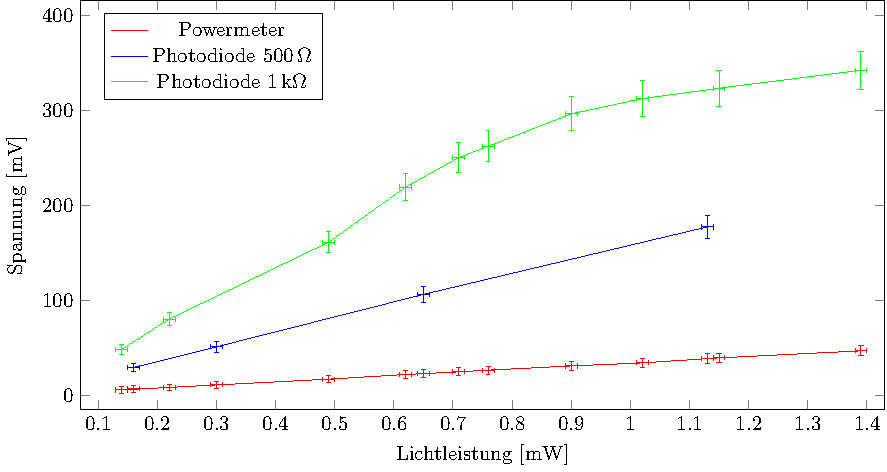
\includegraphics[width=1\linewidth]{graphs/fotodiode/diode.pdf}
	\caption[Vermessung einer Photodiode]{
		Spannungen gemessen über je einen zu einer Photodiode parallel geschalteten Widerstand mit 500 und \unit[1000]{$\Omega$}. Zusätzlich ist der Verlauf der Spannung eines Powermeters aufgetragen.
	}
	\label{fig:photodiode}
\end{figure}

Es ist für \unit[1]{$k\Omega$} eine Sättigung ab etwa \unit[0,9]{mW} erkennbar, die Variante mit \unit[500]{$\Omega$} weist im gesamten Messbereich ein sehr lineares Verhalten auf. Die Fehlerbalken in der x-Achse wurden zu \unit[0,01]{mW} gewählt, da das Powermeter nur zwei Nachkommastellen anzeigt. Der Fehler in der y-Achse wurde auf etwa 5\% gewählt.

%Bei dieser Wellenlänge hat die Photodiode eine Effizienz von etwa \unit[20]{\%} bei der Umwandlung von Licht zu Strom. Bei \unit[660]{nm} (Frequenz des Lasers) etwa \unit[40]{\%}.

	\subsection{4f-Aufbau}
	% !TeX root = ../praktikum.tex
% !TeX encoding = UTF-8
% !Tex spellcheck = de_DE

Im letzten Versuchsteil wurde der Laserstrahl am anderen Ende der Glasfaser ausgekoppelt und auf einen optischen Pfad gesandt, um Abbildungen von Objekten und deren Fourierspektren, sowie die Veränderung der Abbildung bei Maniplation des Fourierspektrums zu beobachten. Hierfür wurde hinter dem Faserauskoppler der Aufbau aus Abbildung \ref{fig:4f-aufbau} realisiert.

\begin{figure}[h]
	\centering
	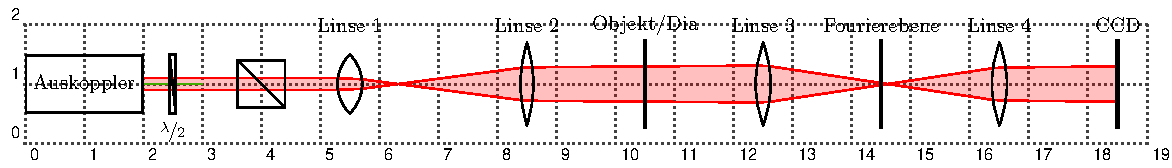
\includegraphics[width=1\linewidth]{graphs/versuchsaufbau/4f-aufbau.pdf}
	\caption[Schematische Skizze des 4f-Aufbaus]{
		Schematische Skizze des 4f-Aufbaus. Der Laserstrahl passiert nach Verlassen des Auskopplers eine $\nicefrac{\lambda}{2}$-Platte und anschließend einen Strahlteiler. Der zweite Teil des Strahls, welcher vom Strahlteiler abgelenkt wird, trifft auf eine Strahlblockierung und wird nicht weiter verwendet. Zwischen Linse 2 und 3 befindet sich die Halterung für das Objekt/Dia, in der Fourierebene wird entweder eine zweite Kamera oder ein Filter positioniert. Die CCD Kamera am Ende des Strahlengangs befindet sich in der Abbildungsebene des Aufbaus.
	}
	\label{fig:4f-aufbau}
\end{figure}

In diesem sogenannten 4f-Aufbau passierte der Laserstrahl nach der Reflektion am ersten Spiegel eine $\nicefrac{\lambda}{2}$-Platte und dahinter einen Strahlteiler. Mit Hilfe des Strahlteilers wurde eine eindeutige Polarisierung sicher gestellt, während mit dem Plättchen die Lichtmenge der durchlässigen Polarisation eingestellt werden konnte.\\

Um die abzubildenden Objekte vollständig ausleuchten zu können, wurde der Laserstrahl in diesem Aufbau mit Hilfe der ersten beiden Linsen aufgeweitet und wieder kollimiert. Im Brennpunkt der dritten Linse befand sich ein Objektträger in der Gegenstandsebene. In diesem wurden die abzubildenden Objekte angebracht. Die Fourierebene befindet sich im Brennpunkt der Linsen 3 und 4. Nach der vierten Linse wird der Strahl erneut kollimiert und trifft auf die CCD Kamera, Kamera 1. Hier wird das Objekt möglichst originalgetreu abgebildet. Um Aufnahmen der Fourierspektren zu erhalten, wurde bei Bedarf eine zweite Kamera, Kamera 2, in der Fourierebene montiert. \\ 

Verwendet wurden hierbei Linsen der Brennweiten wie folgt: Linse 1 mit $f_{1}=\unit[20]{mm}$, Linse 2 mit $f_{2}=\unit[200]{mm}$, Linse 3 und 4 mit $f_{3}=f_{4}=\unit[100]{mm}$. Direkt hinter der Auskopplung wurde zusätzlich ein Spiegel, optimiert für Wellenlängen von \unit[400-700]{nm}, in den 4f-Aufbau aufgenommen, um den Verlauf des Laserstrahls im optischen Pfad besser feinjustieren zu können. Leider wurde die Strahlqualität durch diesen stark beeinträchtigt, so dass zusätzlich ein Pinhole zwischen Linse 1 und 2 notwendig war, um eine gaußähnliche Strahlmode zu erhalten.\\


\begin{figure}[h]
	\centering
	\includegraphicsRS[width=0.7\linewidth][.7]{images/4f-anfang.JPG}
	\caption[Vorderer Teil des 4f-Aufbaus]{
		Vorderer Teil des realisierten 4f-Aufbaus. \textbf{Hintere Reihe, von links nach rechts:} Faserauskoppler; Strahlblockade für den im Strahlteiler reflektierten Anteil. \textbf{Vordere Reihe, von links nach rechts:} zusätzlich eingebauter Spiegel; $\nicefrac{\lambda}{2}$-Platte; Strahlteiler; Diahalter; Linse 1; Pinhole, welches am rechten Bildrand hinter Linse 1 zu sehen ist.
	}
	\label{fig:_DSC7961}
\end{figure}

\begin{figure}[ht]
	\centering
	\includegraphicsRS[width=0.43\linewidth][.45]{images/_DSC7988.JPG}~
	\includegraphicsRS[width=0.43\linewidth][.45]{images/IMG_2223.jpg}
	%\vspace{2cm}\hspace{2cm}
	\caption[Mode vor und nach Verwendung eines Pinholes]{
		\textbf{Links:} Mode des Laserstrahls am Ende des optischen Pfades vor Einbau des Pinholes.\\
		\textbf{Rechts:} Mode des Laserstrahls am Ende des optischen Pfades nach Einbau des Pinholes.
	}
	\label{fig:_DSC7988}
\end{figure}


Als Hilfsmittel bei der Justage des 4f-Aufbaus wurde hier eine Iris verwendet. Mit dieser konnte beispielsweise die Kollimierung des Laserstrahls hinter Linse 2 Überprüft werden, indem die Öffnung der Iris auf die Strahlbreite eingestellt wurde und anschließend entlang des optischen Pfades verschoben wurde. Dabei konnte überprüft werden, ob die Breite des Laserstrahls konstant blieb. Die Justage der Linse konnte somit verbessert werden. Außerdem ließ sich mit Hilfe der Iris über die gleiche Vorgehensweise die Höhe des Strahls entlang des gesamten 4f-Aufbaus kontrollieren und diese dann mit Hilfe der Technik des Walkens optimieren. 


\begin{comment}
\begin{figure}
	\centering
	\includegraphicsRS[width=0.7\linewidth, angle=90]{images/_DSC7967.JPG}
	\caption{Foto des hier realisierten 4f-Aufbaus.}
	\label{fig:_DSC7967}
\end{figure}
\end{comment}

\clearpage



	\label{chap:abb+ft}
		
		
	\section{Experimentelle Durchführung und Auswertung}
	\label{chap:auswertung}
	In diesem Teil sollen Bildinformationen eines Objektes fouriertransformiert, die Transformierte aufgenommen, mit Hilfe verschiedener Filter manipuliert und anschließend rücktransformiert werden. Hierfür werden Objekte, wie z.B. Dias in die Objektebene eingebracht. In der Fourierebene können  Filter oder eine Kamera montiert werden, um die Fouriertransformierte manipulieren oder aufnehmen zu können. Eine Kamera dient zur Aufnahme der Rücktransformierten.\\
	
	Die fünf verwendeten Objektdias werden als \textit{Objekte 1 bis 5} (siehe Abbildung~\ref{fig:Objekte-aus-Anleitungsheft}) bezeichnet. Objekt 1-4 enthalten mehrere Motive, die einzeln untersucht werden.
	
	\begin{figure}[h]
		\centering
		\includegraphicsRS[width=0.15\textwidth][.15]{images/Anleitungsheft/objekt1.png}~~
		\includegraphicsRS[width=0.15\textwidth][.15]{images/Anleitungsheft/objekt2.png}~~
		\includegraphicsRS[width=0.15\textwidth][.15]{images/Anleitungsheft/objekt3.png}~~
		\includegraphicsRS[width=0.15\textwidth][.15]{images/Anleitungsheft/objekt4.png}~~
		\includegraphicsRS[width=0.15\textwidth][.15]{images/Anleitungsheft/objekt5.png}
		\caption[Die zur Messung verwendeten Diamotive]{
			Darstellung der zur Messung verwendeten Dias. Im Text werden diese Objektdias mit Objekt 1 bis 5, von links nach rechts, bezeichnet.
		}
		\label{fig:Objekte-aus-Anleitungsheft}
	\end{figure}
	
	Anhand der Dias wurden zunächst sowohl Kamera 1, als auch Kamera 2 nachjustiert, bis ein möglichst scharfes Bild auf dem über das Programm \textit{uc480 Viewer-DCC1545M-ID} angeschlossenen Bildschirm zu erkennen war. %In den nachfolgenden Teilen werden für die Objekte Aufnahmen in der Abbildungsebene und zugehörig zu jeder Einstellung auch in der Fourierebene gemacht. Zudem werden für die Objekte 4 und 5 verschiedene Filter in die Fourierebene gestellt und Aufnahmen der Kamera 1 in der Abbildungsebene gemacht und untersucht. Für Objekt 4 wurde hierzu ein Tiefpass und mehrere Breitbandfilter verwendet. Für Objekt 5 wurde ein Halbebenenfilter horizontal, vertikal und diagonal in die Fourierebene gehalten.\\
		
	% !TeX root = ../praktikum.tex
% !TeX encoding = UTF-8
% !Tex spellcheck = de_DE



\subsection{Untersuchungen an Gittern}
In diesem Abschnitt werden verschiedene Gitter des Objektes 3 untersucht. Dazu wurde das entsprechende Dia in der Objektebene montiert. Das gewünschte Motiv auf der Schablone wurde möglichst mittig in dem Strahl montiert. Mit einer Papierschablone wurde verhindert, das Motive beleuchtet werden, die gerade nicht untersucht wurden, da dies eine Überlagerung mehrerer Fourierspektren zur Folge hätte (vgl. Abb.~\ref{fig:kreuzgitter_und_spektrum}~a und b) und das Untersuchen eines einzelnen Spektrums unmöglich machen würde. Für jedes der neun Motive wurde je ein Bild in der Fourierebene sowie in der Abbildungsebene aufgenommen. Bei dem Einschieben der Objekte lässt sich feststellen, dass die Bewegungsrichtung der Abbildung entgegengesetzt zu der des echten Motives ist. Ebenso sieht man bei asymmetrischen Objekten, dass diese "auf dem Kopf stehen".


\begin{figure}[ht]
	\centering
	%\includegraphicsRS[width=0.6\textwidth]{images/Regina/abb13.jpg}
	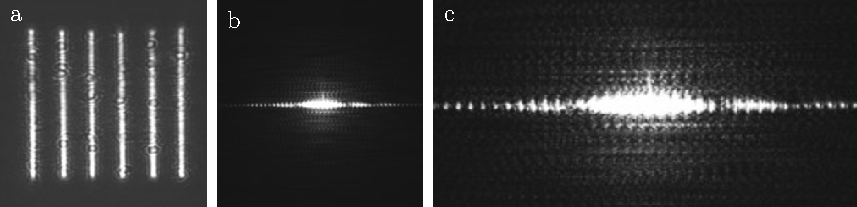
\includegraphics{images/Regina/abb13.pdf}
	\caption[Gitter mit Fourierspektrum]{
		Vertikales Gitter (a) und das dazugehörige Beugungsbild (b), welches das Fourierspektrum darstellt. Das Fourierspektrum weist erneut Beugungsbilder als eine Unterstruktur auf (c).
	}
	\label{fig:gitter_und_spektrum}
\end{figure}

Für eines der Gittermotive aus der ersten Reihe sind diese Aufnahmen in Abbildung~\ref{fig:gitter_und_spektrum} abgebildet. In der Fourierebene ist eine Reihe von Punkten zu sehen. Die Motive der zweiten Reihe ergeben in beiden Ebenen jeweils das gleiche Bild, jedoch um $90^\circ$ gedreht. Je dichter die Gitterlinien beieinander liegen, desto weiter liegen die Punkte in der Fourierebene auseinander.

Die Abbildung eines Motiv der letzten Reihe (Kreuzgitter) ist in Abbildung~\ref{fig:kreuzgitter_und_spektrum}~a abgebildet, b zeigt das Bild in der Fourierebene (\textit{Fourierspektrum}). Zusätzlich zeigt die Abbildung~\ref{fig:kreuzgitter_und_spektrum}c das Fourierspektrum, wenn mehrere Motive gleichzeitig beleuchtet werden. Die Kreuzgitter erzeugen in der Fourierebene zwei senkrechte Punktreihen, wobei der Punktabstand mit zunehmenden Gitterlinienabstand abnimmt.

\begin{figure}[ht]
	\centering
	%\includegraphicsRS[width=0.4\textwidth]{images/Regina/abb14.jpg}
	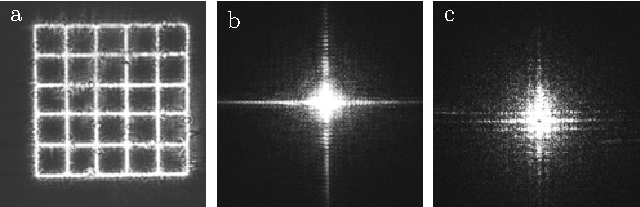
\includegraphics{images/Regina/abb14.pdf}
	\caption[Kreuzgitter mit Fourierspektrum]{
		Kreuzgitter (a) und das dazugehörige Beugungsbild (b), das das Fourierspektrum darstellt. Eine Überlagerung von mehreren Fourierspektren (c).
	}
	\label{fig:kreuzgitter_und_spektrum}
\end{figure}



\subsubsection*{Auswertung}
Das Zustandekommen und Aussehen einer Abbildung kann durch die aus der zweifachen 
Da das Licht im vertikalen Gitter nur in der vertikalen Richtung gebeugt wird, bilden sich die Intensitätsschwankungen in der Fourierebene ausschließlich in horizontaler Richtung aus. Somit wurde dort eine senkrecht zu dem Gitter stehende Reihe aus Interferenzmaxi- und -minima beobachtet: Vergleich Abbildung~\ref{fig:gitter_und_spektrum}. Das Drehen des Motives sorgt ebenfalls für ein gedrehtes Bild in der Fourierebene. Dies ist direkt aus der Beugungstheorie an Gittern ersichtlich. Die Änderungen des Spektrums unter Variation des Spaltabstandes zu beobachten waren, lassen sich mit der mathematischen Eigenschaft der Ähnlichkeit der FT erklären (s. Abschnitt~\ref{chap:math_basic}), allerdings folgt auch dies direkt aus der Beugungstheorie an Gittern beziehungsweise Mehrfachspalten.\\

Bei einem Kreuzgitter findet die Beugung in horizontaler und vertikaler Richtung statt, welches einer Kreuzform in der Fourierebene entspricht. Das Motiv entspricht also einer Überlagerung zweier um $90^\circ$ gedrehten Gitter. Nach der mathematischen Eigenschaft der Linearität der FT (s. Abschnitt~\ref{chap:math_basic}) folgt somit auch die Überlagerung der entsprechenden Spektren. Dies war sehr gut zu beobachten.

Wenn mehrere Motive beleuchtet wurden ergab sich in der Fourierebene die in Abbildung~\ref{fig:kreuzgitter_und_spektrum}~c dargestellt kreuzförmige Anordnung. Diese zeigt nicht ein einzelnes Kreuz, sondern mehrere Kreuze mit einem bestimmten Abstand voneinander. Das Auftreten mehrerer Kreuze lässt sich analog mit der Linearitätseigenschaft der FT erklären.

Sowohl bei dem vertikalen Gitter als auch bei dem Kreuzgitter ist in der Fourierebene im Zentrum der Beugungsbilder eine maximale Intensität zu erkennen. Dieses Maximum entsteht durch das Kreuzen der mittleren horizontalen oder im Kreuzgitter der vertikalen und
horizontalen Beugungsbilder. Dabei ist bei jedem weiteren Kreuzpunkt erneut eine erhöhte Intensität zu erkennen, die aber nach außen hin abnimmt. Diese lässt sich ebenfalls bei einem
Doppelspalt beobachten, wobei das Intensitätsmaximum nullter Ordnung am stärksten ist und die Maxima höherer Ordnungen immer schwächer werden ($\nicefrac{sin(x)}{x}$). Dabei nimmt die Intensität im Zentrum mit zunehmen kleiner werdenden Gitterkonstante zu.
Weiterhin wiesen alle Intensitätsmaxima eine Unterstruktur auf. Diese Unterstrukturen entstehen durch die Interferenz der Haupt- und Nebenmaxima aller Spalte des Gitters. Somit entsteht im Gegensatz zu einem Doppelspalt das Beugungsbild eines Gitter aus Vielfachinterferenzen. Diese Eigenschaft entspricht der mathematischen geforderten Linearität. Denn das Beugungsbild eines Gitters kann somit durch das aufsummieren der einzelnen Beugungsbilder des Einzelspaltes erzeugt werden (siehe 1.1. Linearität%TODO:REF!!!
).


\subsection{Erzeugung von Beugungsbilder von Punkten}
\subsubsection*{Auswertung}

Bei der optische Fouriertransformation gilt für Punkte wie bereits für Gittern erläutert die Linearität, so dass das erzeugte Beugungsbild in der Fourierebene sich aus der Summe der Beugungsbilder der einzelnen Punkte ergibt. Das Beugungsbild eines Punktes besteht aus konzentrischen Ringen, dessen Breite und Intensität nach außen abnehmen. Durch das Verschiebungtheorem der Fouriertransformation ist gegeben, dass sich das Beugungsbild der beiden Punkte an einer Position befinden, trotz der unterschiedlichen Position der Punkte. Bei zwei Punkten ergibt sich somit erneut eine Vielfachinterferenz analog zum Gitter, welches erneut durch Unterstrukturen in den konzentrischen Ringen erkennbar wird (Abb.~\ref{fig:punktpaare_verschieden_und_spektren}~b, d). Mit zunehmenden Abstand zwischen den Punkten werden die Unterstrukturen feiner. Dieses entspricht dem Ähnlichkeitstheorem (siehe 1.1. Ähnlichkeit%TODO:REF!!!
), so dass mit zunehmenden Abständen der Punkte sich die Beugungsmaxima annähern, bzw. die Abstände zwischen diesen kleiner werden. Für ein Gitter bedeutet dieses, je größer die Gitterkonstante ist, d.h. je größer der Abstand zwischen den Spalten ist, desto kleiner wird der Abstand zwischen den einzelnen Maxima und Minima.

\begin{figure}[h]
	\centering
	%\includegraphicsRS[width=0.3\textwidth]{images/Regina/abb15.jpg}
	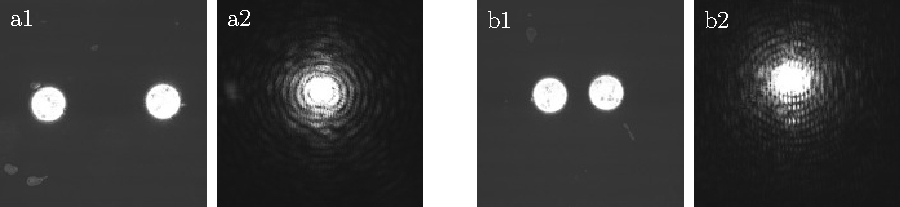
\includegraphics{images/Regina/abb15.pdf}
	\caption[Punktpaare unterschiedlicher Abstände und Fourierspektren]{
		Punktpaare mit unterschiedlichen Abständen zueinander (a1, b1) und die dazugehörigen Beugungsbilder in der Fourierebene (a2, b2).
	}
	\label{fig:punktpaare_verschieden_und_spektren}
\end{figure}


\begin{figure}[h]
	\centering
	%\includegraphicsRS[width=0.3\linewidth]{images/Regina/abb16.jpg}
	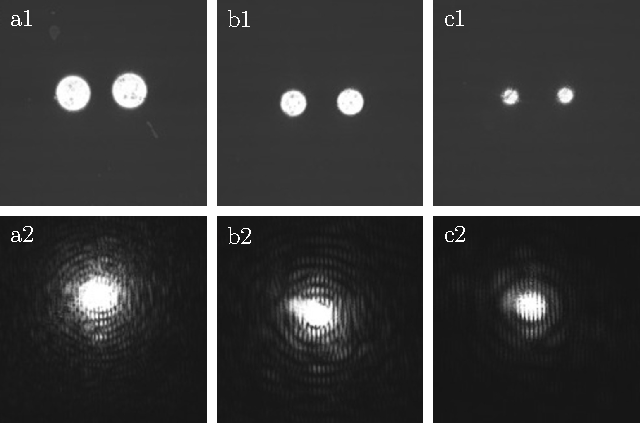
\includegraphics{images/Regina/abb16.pdf}
	\caption[Punktpaare gleicher Abstände und Fourierspektren]{
		Punktpaare mit gleichen Abständen und unterschiedlicher Größe (a1, b1, c1) und die dazugehörigen Beugungsbilder in der Fourierebene (a2, b2, c2).
	}
	\label{fig:punktpaare_gleich_und_spektren}
\end{figure}

Bei den geringsten Abstand sind im Beugungsbild neben den konzentrischen Formen auch vertikale Gitter zu erkennen (Abb.~\ref{fig:punktpaare_verschieden_und_spektren}~b2). Diese Gitterform stellen die bereits erwähnten Unterstrukturen der Beugungsbilder dar. Zwei Punkte ergeben in der Fourierebene als
Unterstruktur eine Linienstruktur senkrecht zur Verbindungslinie der beiden Punkte. Diese ergeben sich somit ebenfalls bei zwei Punkten mit höheren Abstand, sind aber wegen des kleinen Abstand zwischen den Spalten des vertikalen Gitters in der Fourierebene schlecht zu erkennen, da sich die Fouriertransformierte reziprok verhält (Ähnlichkeitstheorem). Bei kleinere Abstand zwischen den Punkten, vergrößert sich der Abstand der Spalten im vertikalen Gitter, und ist dadurch erkennbar. Diese Unterstrukturen sind noch ausgeprägter bei gleichbleibenden Abstand und kleinerer Größe der Punkte zu erkennen (Abb.~\ref{fig:punktpaare_gleich_und_spektren}~b2, c2). Die Intensitätsmaxima sind bei den kleineren Punkte durch ihren größeren Abstand zueinander kleiner ausgeprägt als bei den größeren Punkten. Somit weist das Hauptmotiv des Beugungsbild eine geringe Intensität auf, wodurch die Unterstruktur einfacher zu erkennen
ist.
Auch bei dem Beugungsbild eines Punktringes (Abb.~\ref{fig:punktringe_und_spektrum}) sind Unterstrukturen in der Fourierebene zu erkennen, die sich durch die Anordnung der acht Punkte ergeben. Zwei Punkte weisen eine senkrechte Linienstruktur zur Verbindungslinie auf, so dass sich bei acht Punkten vier Linienstrukturen (horizontal, vertikal, beide Diagonale) ergeben. Wenn sich diese Strukturen kreuzen, ergeben sich acht Schnittpunkte und somit eine Unterstrukturen, die wie Achtecke aussehen (Abb.~\ref{fig:punktringe_ausschnitt}).

\begin{figure}[h]
	\centering
	%\includegraphicsRS[width=0.10\linewidth]{images/Regina/abb17.jpg}
	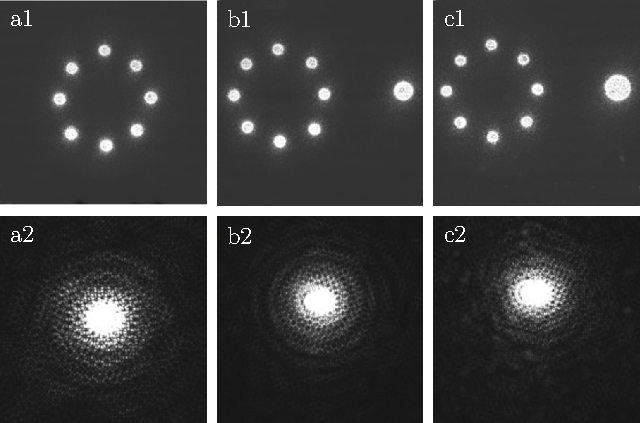
\includegraphics{images/Regina/abb17.pdf}
	\caption[Punktringe mit Fourierspektren]{
		Punktringe (a1) und Punktringe mit zusätzlichem Punkt in unterschiedlicher Größe (b1, c1) und die dazugehörigen Beugungsbilder in der Fourierebene (a2-c2).
	}
	\label{fig:punktringe_und_spektrum}
\end{figure}

\begin{figure}[h]
	\centering
	\includegraphicsRS[width=0.42\textwidth]{images/Regina/abb18.jpg}
	\caption[Beugungsbild der Punktringe mit vergrößertem Ausschnitt]{
		Ausschnitt aus dem Beugungsbild des Punktringes, welche die Unterstruktur eines Achtecks zeigt.
	}
	\label{fig:punktringe_ausschnitt}
\end{figure}

Bei einem Punktkreis mit einem zusätzlichen Punkt ist das Beugungsbild nicht mehr symmetrisch und die Asymmetrie nimmt mit größer werdenden Punkt zu (Abb.~\ref{fig:punktpaare_gleich_und_spektren}~b, c).


\subsection{Erzeugung von Beugungsbilder von Buchstaben und Zahlen}
\subsubsection*{Auswertung}

Der Buchstabe D besteht aus sowohl horizontalen, vertikalen Linien und runden Elementen (Abb.~\ref{fig:ziffern_mit_spektren}~a1). Das Beugungsbild ergibt sich somit aus der Summe der Beugungsbilder dieser verschiedenen Formen. Die horizontalen Linien bilden ein Fourierspektrum in der Horizontalen und die vertikalen Linien in der Vertikalen mit den jeweiligen Maxima und Minima und Unterstrukturen (Abb.~\ref{fig:ziffern_mit_spektren}~a2). Die runde Form erzeugt in dem Beugungsbild konzentrische Ringe mit abnehmender Intensität, entsprechend dem Beugungsbild von Punkten. Da der Buchstabe D durch horizontale und vertikalen Linien dominiert wird, ist auch das Beugungsbild stark davon geprägt, so dass die konzentrischen Ringe durch eine geringere Intensität auch schlechter zu erkennen sind.

\begin{figure}[h]
	\centering
	%\includegraphicsRS[width=0.4\textwidth]{images/Regina/abb19.jpg}
	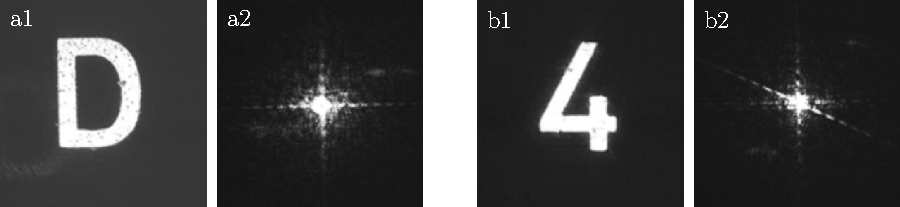
\includegraphics{images/Regina/abb19.pdf}
	\caption[Ziffern mit Fourierspektren]{
		Buchstabe D (a1) und Zahl 4 (b1) und die dazugehörigen Beugungsbilder in der Fourierebene (a2 und b2).
	}
	\label{fig:ziffern_mit_spektren}
\end{figure}

Die Zahl 4 besteht lediglich aus Linien, wobei neben horizontalen und vertikalen Linien ebenfalls diagonale Linien vorhanden sind (Abb.~\ref{fig:ziffern_mit_spektren}~b1). Da das erzeugten Beugungsbild eines Gitters eine senkrecht auf dem Gitter stehende Punktereiche aus Interferenzmaxima und –minima darstellt, ist zusätzlich zu der horizontalen und vertikalen Richtung ein Fourierspektrum in der Diagonalen senkrecht zur der Diagonale der Objektebene anzufinden (Abb.~\ref{fig:ziffern_mit_spektren}~b2).

\subsection{Erzeugung von Beugungsbildern des Fourierhauses}
\subsubsection*{Auswertung}

Das Fourierhaus ist ein Haus, welches aus Gittern mit gleichen Gitterkonstanten und unterschiedlicher Ausrichtungen der Gitter besteht (Abb.~\ref{fig:fourierhaus_mit_filtern}~a1). Die verschiedenen Gitter entsprechen verschiedenen Bauelementen im Haus. Die Wand besteht aus einem vertikalen Gitter, das Dach aus einem horizontalen Gitter und die Tür und der Schornstein werden aus diagonalen Gittern in entgegen gerichteten Richtung erstellt. Die Fouriertransformation dieses Fourierhauses ergibt das in Abbildung~\ref{fig:fourierhaus_mit_filtern}a2 dargestellte Beugungsbild. Die vier verschiedenen Orientierung der Gitter sind in der Fourierebene ebenfalls durch vier verschiedene Orientierungen dargestellt, die jeweils senkrecht auf der Objektebene stehen. Da die Gitterkonstante des Fourierhauses im Vergleich zu den in Abbildung~\ref{fig:gitter_und_spektrum} und \ref{fig:kreuzgitter_und_spektrum} gezeigten Gittern sehr viel kleiner ist, sind die Abstände zwischen den Maxima im Fourierspektrum deutlich größer (siehe 1.1. Ähnlichkeit%TODO REF!!!
 ) und die Intensität im Zentrum erhöht.


\subsection{Optische Filterung des Fourierhauses durch eine Schneide}
\subsubsection*{Auswertung}

Für eine optische Filterung wurden verschiedene Filter in der Fourierebene des 4f-Aufbaus eingesetzt (siehe Abb.4%TODO:REF!!!
). Zuerst wurde das Fourierhaus durch Filter manipuliert. Durch die Verwendung einer Schneide, die bestimmte Frequenzbereiche durch das Abdecken der Frequenzspektren durch lichtundurchlässigen Material herausfiltert, konnten verschieden Bauelemente jeweils heraus gefiltert werden. Durch zwei Schneiden wurden in dem Fourierebene das Beugungsbild so abgedeckt, dass lediglich das vertikale Fourierspektrum des Daches und das diagonale Fourierspektrum der Tür übrig blieben (Abb.~\ref{fig:fourierhaus_und_spektrum}~b1). Somit waren in der Abbildungsebene nur die näherungsweise horizontalen Linien des Daches und der Tür sichtbar (Abb.~\ref{fig:fourierhaus_und_spektrum}~b2). Analog wurden durch das Abdecken mit dem Filter erreicht, dass nur das horizontale Fourierspektrum sichtbar war und somit nur vertikale Linien (Wand) in der Abbildungsebene sichtbar wurden (Abb.~\ref{fig:fourierhaus_und_spektrum}~c1, c2). Als letztes wurde, durch das Blockieren des diagonalen Fourierspektrums, lediglich der Schonstein ausgeblendet (Abb.~\ref{fig:fourierhaus_und_spektrum}~d1, d2).

\begin{figure}[h]
	\centering
	%\includegraphicsRS[width=0.75\textwidth]{images/Regina/abb21.jpg}
	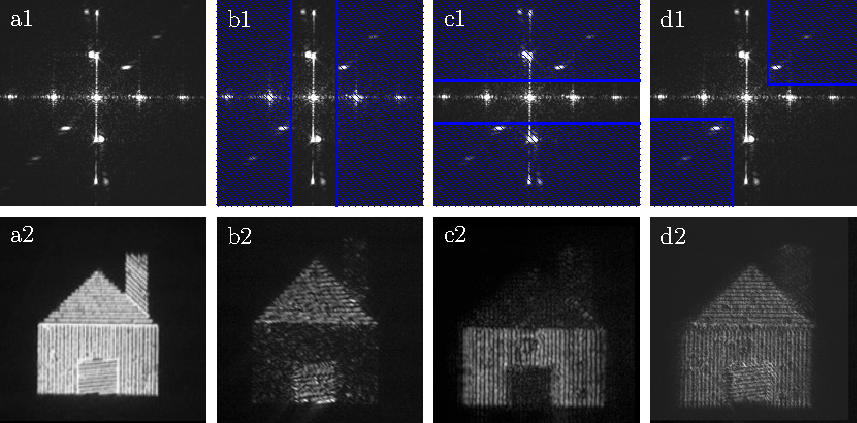
\includegraphics[scale=1]{images/Regina/abb21.pdf}
	
	\caption[Fourierhaus mit verschiedenen Filtern]{
		Durch zwei Schneiden (blau schraffiert) werden verschiedene Teile der Fourierspektren in der Fourierebene herausgefiltert (oben), welches in der Abbildungsebene zum Verschwinden einzelner Teile führt (unten).
	}
	\label{fig:fourierhaus_mit_filtern}
\end{figure}

\subsection{Optische Filterung durch Hochpass-, Tiefpass- und Breitbandfilter}

Als Nächstes wurde die Abbildung eines Fingerabdrucks auf einem Glasplättchen zunächst ohne Filter aufgenommen. Hierbei war in der Abbildungsebene relativ wenig zu erkennen (siehe Abbildung \ref{fig:example20_Hochpass}~a). Anschließend wurde die Abbildung mit einem in der Fourierebene befindlichen Hochpass- und einem Halbebenenfilter aufgenommen. Zudem wird mit Kamera 2 das Fourierspektrum des Fingerabdrucks photographiert. Zu beobachten war hier, dass die Konturen des Fingerabdrucks in der Abbildung mit Hilfe der Filter deutlich besser erkennbar gemacht werden konnten (vgl Abbildung \ref{fig:example20_Hochpass}~b, c).\\


\begin{figure}[h]
	\centering
	%\includegraphicsRS[width=0.6\linewidth]{images/example20_Hochpass.png}\\
	%\includegraphicsRS[width=0.6\linewidth]{images/example21_Halbebenenfilter.png}
	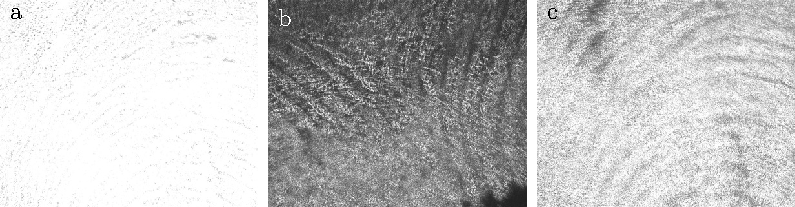
\includegraphics{images/ergebniss_Fingerab/abb.pdf}
	%TODO: Nur eines dieser Bilder!
	\caption{
		Der Fettabdruck eines Fingers in der Abbildungsebene ohne Filter (a) und mit Hochpassfiltern (b, c).
	}
	\label{fig:example20_Hochpass}
\end{figure}

\subsubsection*{Auswertung}

Als Erstes wird ein Breitbandfilter bei der Zahl vier eingesetzt. Da der Breitbandfilter sowohl kleinere und größere Frequenzen herausfiltert und somit nur eine bestimmtes Frequenzintervall durchlässt, werden die Flächen unterdrückt und Ränder als Doppellinien dargestellt. Beim Breitbandfilter C (Abb %TODO REF!!!
c) konnte dieser Effekt am besten beobachtet werden (Abb.~\ref{fig:vier_mit_breitband}~b). Bei den Breitbandfilter B und A ist die Filterwirkung so stark, dass nur
ein sehr kleiner Frequenzintervall durchgelassen wird und dadurch die Zahl vier kaum noch zu erkennen ist (Abb. \ref{fig:vier_mit_breitband}c, d).

\begin{figure}[h]
	\centering
	%\includegraphicsRS[width=0.4\textwidth]{images/Regina/abb22.jpg}
	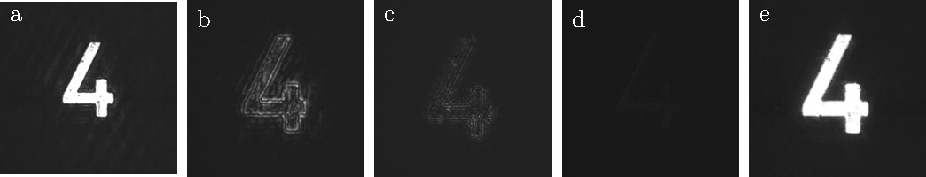
\includegraphics{images/Regina/abb22.pdf}
	\caption[Zahl 4 mit Breitbandfiltern]{
		Die Zahl vier in  der Abbildungsebene ohne Filter (a) und mit dem Breitbandfilter C (b), B (c) und A (d) gefilterte Bilder der Zahl vier.
	}
	\label{fig:vier_mit_breitband}
\end{figure}

Durch die Verwendung eines Tiefpassfilters wurden die niedrigen Frequenzen durchgelassen und somit die hohen Frequenzen herausgefiltert. Diese bewirken eine niedrigere Auflösung des
Bildes, da die Flächen unterdrückt werden, welches in der Abbildung~\ref{fig:vier_mit_breitband}~b dargestellt ist bei der Zahl 4 und dem Buchstaben D dargestellt ist. Da diese beiden Objekte keine innere Flächenstrukturen wie Gitter aufweisen, ist dieser Effekt nicht zu erkennen.
Im Gegenteil dazu wurden bei einem Fingerabdruck ein Hochpassfilter eingesetzt, der die niedrigen Frequenzen herausgefiltert, welches zu einer Hervorhebung der Kanten führte (Abb.~\ref{fig:vier_mit_tiefpass}~b). In der Bildverarbeitung werden die Tiefpass- (Weichzeichner) und Hochpassfilter (Kantenerkennung) häufig verwendet.

\begin{figure}[h]
	\centering
	%\includegraphicsRS[width=0.4\textwidth]{images/Regina/abb23.jpg}
	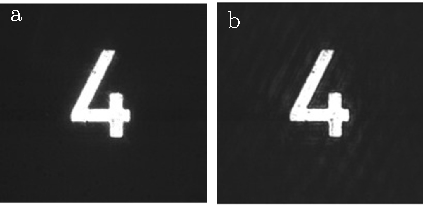
\includegraphics{images/Regina/abb23.pdf}
	\caption[Zahl 4 mit Tiefpassfilter]{
		Die Zahl vier in der Abbildungsebene (a) und mit dem Tiefpassfilter (b) gefilterte Abbildung der Zahl vier.
	}
	\label{fig:vier_mit_tiefpass}
\end{figure}


\begin{figure}[h]
	\centering
	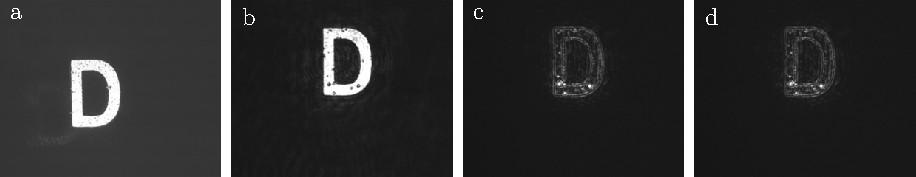
\includegraphics{images/ergebniss_D/abb.pdf}
	\caption{
		Der Buchstabe D des Objekts 4 in der Abbildungsebene ohne Filter (a), mit dem Filter 1D (b), 1C (c), 1B (d).
	}
	\label{fig:example10_Filter1B}
\end{figure}


\subsection{Schlierenverfahren durch Verwendung eines Halbebenenfilters}

Als Letztes wurde ein Teelicht auf die Position des Objektträgers gestellt und ein Halbebenenfilter in der Fourierebene installiert. Mit Kamera 1 wurden mehrere Abbildungen aufgenommen, um die Strömungsbewegungen oberhalb der Flamme beobachten zu können. Zum Vergleich wurde zudem eine Aufnahme mit Halbebenenfilter, jedoch ohne Teelicht gemacht (siehe Abb.~\ref{fig:Halbebenenfilter_mit_und_ohne_Teelicht}). Auf dieser Beispielaufnahme sind deutliche Verzerrungen des Lichts aufgrund der Luftströmungen über der Flamme des Teelichts zu erkennen. 

\begin{figure}[h]
	\centering
	%\includegraphicsRS[width=0.7\linewidth]{images/example22_Halbebenenfilter_mit_und_ohne_Teelicht.png}
	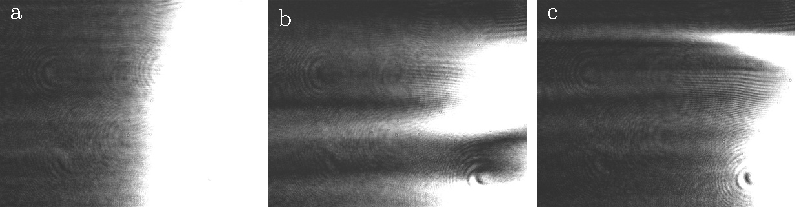
\includegraphics{images/ergebniss_Teelicht/abb.pdf}
	\caption[Schlieren]{
		Aufnahme ohne Objekt in der Abbildungsebene mit Halbebenenfilter ohne Teelicht (a) und mit Teelicht (b, c).
	}
	\label{fig:Halbebenenfilter_mit_und_ohne_Teelicht}
\end{figure}


\subsubsection*{Auswertung}

Mit Hilfe eines Halbebenenfilters (Schneide) wurden die durch   eine brennende Kerze erzeugten Schlieren dargestellt (Abb.~\ref{fig:Halbebenenfilter_mit_und_ohne_Teelicht}). Als Schlieren werden Bereiche bezeichnet, die sich von ihrer Umgebung  in  der  Dichte  bzw.  im  Brechungsindex  unterscheiden,  welche  in  unseren Versuch die durch  die  Kerze erzeugten Luftströmungen darstellten. Bei diesem Versuchsaufbau  wurde  das  Prinzip  genutzt,  dass  parallele  Strahlenbündel  beim  Durchgang durch   ein   inhomogenes Dichtefeld   unterschiedlich   stark   abgelenkt   werden.   Durch   die eingesetzte  Schneide,  wurden  die  Anteile  des  gebrochenen  Lichts  ausgeblendet,  so  dass richtungsabhängige  Brechzahl-  bzw.  Dichtegradienten auf  dem  Projektionsschirm  sichtbar wurden. Dabei ist die Intensitätsverteilung im   Bild   proportional   zum   Quadrat   der Phasenverschiebung   durch   das   Objekt.   Somit   ermöglicht es dieses Verfahren, eine Phasenverschiebung sichtbar zu machen. 

	
	\clearpage
	\newpage
	
	\section{Fazit} %Diskussion der physikalischen Ergebnisse
	% !TeX root = ../praktikum.tex
% !TeX encoding = UTF-8
% !Tex spellcheck = de_DE



Durch diesen Versuch werden die theoretischen mathematischen Grundlagen der Fouriertransformation anhand anschaulicher Experimente nachvollziehbar. Dabei ist der Vergleich der Eigenschaften der Linse und dem entsprechenden Aufbau mit den geforderten. Eigenschaften einer Funktion (Linearität, Ähnlichkeit, Verschiebung, Faltung) für eine Fouriertransformation für das Verständnis sehr nützlich. Insbesondere wird dies durch die Verwendung von verschiedenen Filtern und die daraus folgende Manipulation der Bilder vermittelt. 

Der selbständige Aufbau, der die Optimierung des Diodenlasers als auch des Strahlengangs umfasste, veranschaulichte deutlich die Herausforderungen des Versuchs und somit die Herausforderungen beim Experimentieren und somit dem Umgang mit der Ausrüstung in der Optomechanik. Dabei ist viel Geduld, z.B. bei der Einkopplung erforderlich, sowie auch Kreativität, was uns anhand des Baus der Photodiode zur Messung der Effizienz des Lasers verdeutlicht wurde. Weiterhin zeigte das Justieren des Strahlengangs, dass bereits kleinste Veränderungen einen enormen Einfluss auf die Auflösung der Abbildung haben können.
%Die entstehenden Unterschiede können anhand unserer Abbildungen des Fourierhauses gezeigt werden, die an zwei unterschiedlichen Tagen erzeugt wurden (Abb.19 vgl. Abb. 20%TODO: REF!!!).
Die Wirkung der Filter auf die Abbildungen erhöhte ebenfalls das Verständnis für Effekte, wie Weichzeichner oder Kantenerkennung in der digitalen Bildverarbeitung. Da Filterungen ebenfalls in der Akustik verwendet werden, um z.B. Rauschen herauszufiltern oder zur Kompression von Daten (jpeg, mp3), wurde somit die breite Anwendung der Fouriertransformation anhand des Versuchs der optischen Fouriertransformation verdeutlicht.
	
	\newpage
	\clearpage
	
	%\section{} %Zusammenfassung
	
	
	\newpage
	\clearpage
	
	%\pagenumbering{Roman}
	\pagenumbering{Alph}
	
	
	%\nocite{bibid}
	\addcontentsline{toc}{section}{Literatur}
	\bibliographystyle{deIEEEtran}
	\bibliography{IEEEabrv,praktikum}
	
	\newpage
	
	\addcontentsline{toc}{section}{Abbildungsverzeichnis}
	\listoffigures %lof
	%\tableofcontents %toc
	%\listoftables %lot
	
	\newpage
	\clearpage
	
	\section{Anhang}
	% !TeX root = ../praktikum.tex
% !TeX encoding = UTF-8
% !Tex spellcheck = de_DE

	
\end{document} 